\scanpage{22}
\uline{Rectification} \quad Si $G$ monoïde affine de t.f. sur corps $k$, on a une immersion fermée multiplicatif $G\mathbin{-}\mathbb M_{\unsure{n,k|n\,k}}$ (non $G\to\unsure{GL_{n,k}|Gl_{n,k}}$\unsure{)} car on peut montrer que si $G$ est un monoïde de pres. finie sur un anneau $k$, tel que les translations à g (disons sont des mono) - p.ex. s'il $\exists$ \unsure{mono|un} $G\longrightarrow G'$, $G'$ un \inserted{foncteur en} groupes - alors $\deleted{\unsure{G}}G$ est un objet gr-pe).

\figure{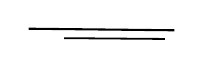
\begin{tikzpicture}[x=1cm,y=1cm]
\draw[line width=.75pt] (0,0) -- (1.85,-.02);
\draw[line width=.65pt] (.45,-.12) -- (1.73,-.13);
\end{tikzpicture}}

\deleted{$G$} $X$ schéma affine sur $k$, \deleted{\unsure{de|et}} de $k$-algèbre $\mathcal A$. On définit $\check{\mathcal A}=\mathrm{Dist}(X\deleted{)},k)$. On \unsure{a|.} le foncteur $\inserted{k'}\rightarrow\mathrm{Dist}(X,k')$, noté $\mathrm{Dis}(X)$, représentable par $\mathbb V(A)$. On a
% slanted
\reversemarginpar\margin{\tikz[baseline=-.3ex,x=1em,y=1em]{\draw[->] (.56,.85) to[out=-130,in=76] (0,-.55);} \uline{covariant}}\normalmarginpar
\[
\left\{\begin{aligned}
&\text{a)}\ \mathrm{Dist}(X)\ \text{fonctoriel en }X\quad
  (\text{comme Module sur }\unsure{\mathcal O|O|\mathbb O}_k)\\
&\text{b)}\ \mathrm{Dist}(X)\times\mathrm{Dist}Y)
  \xrightarrow[\unsure{\pi|\Pi}_{X,Y}]{\deleted{\unsure{\alpha|o}}}
  \mathrm{Dist}(X\times Y)\quad\text{bilinéaire}
\end{aligned}\right.
\]
[et universel pour les hom bilinéaires de $\mathrm{Dis}(X)\times\mathrm{Dis}(Y)$ dans un $\mathbb V(M)$] induisant en fait un isom
\[
\mathrm{Dist}(X)\boxtimes\mathrm{Dist}(Y)\simeq\mathrm{Dist}(X\times Y).
\]

c) On a une inclusion fonctorielle
\[
X\xrightarrow{\alpha_X}\mathrm{Dist}(X)
\]
[distribution ponctuelle, compatible avec passage au produit, i.e. on a comm. des
\diagram{\begin{tikzcd}[ampersand replacement=\&]
X\times Y \arrow[r,"\alpha_X\times\alpha_Y"] \arrow[dr,swap,"\unsure{\pi|\Pi}_{X\times Y}"] \& \unsure{\mathrm{Dist}}(X)\times\mathrm{Dist}(Y) \arrow[d,"\unsure{\pi|\Pi}_{X,Y}"]\\
\& \mathrm{Dist}(X\times Y)
\end{tikzcd}}

\deleted{Si $G$ est muni d'une loi de comp., $\mathrm{Dist}(G)$ aussi. \deleted{\unsure{Si}} Elle est unitaire sss celle de $\mathrm{Dist}(G)$ l'est} En fait on peut rêconstruire $X$ à partir de $\mathrm{Dist}(X)=\mathbb D$ et la structure supplémentaire
\[
D\overset{\Delta}{\unsure{\mathbin{-}|\longrightarrow}}D\boxtimes D
\]
\margin{$[\,V(A)\boxtimes V(B)\overset{\text{def}}{\simeq}V(A\otimes B)\,]$\newline
[NB $\boxtimes=\otimes$ si $A$ ou $B$ proj. de t.f.]}
% slanted
\reversemarginpar\margin{NB on rêconstitue $X$ à partir de $D$ muni \deleted{\unsure{la|du}}de l'application diagonale $D\to D\boxtimes D$ comm. ass. unitaire.}\normalmarginpar
doit être une ``application diagonale'' ass. comm. et counitaire [i.e. on a $D\xrightarrow{\varepsilon}\mathcal O$ \ldots.] comme formé des \deleted{\unsure{pts|gts}} $x\in\mathbb D(k')$ tels que
\[
\boxed{\Delta(x)=x\boxtimes x}
\]
% archive sheet number: 21
